\subsection{Motivation et définition}
	
	Les variables $(u,v)$ de Milne ne sont pas directement reliées aux grandeurs physiques caractérisant la sphère
	isotherme en boîte considérée. Nous utilisons souvent plutôt un autre moyen de représentation issu de la
	thermodynamique et appellé courbe calorique. Cette courbe est en fait directement reliée à celle de Milne et
	consiste à représenter $\mu$ en fonction de $\lambda$ ou de son opposé $-\lambda$ car l'énergie d'un système
	autogravitant est souvent négative. En pratique nous résolvons le système différentiel $u(v)$ en fixant $X$,
	nous déterminons les coordonnées du point extrême $(u_m,v_m)$, puis en utilisant (\ref{uv_max}) nous en déduisons la valeur
	du couple $(\lambda,\mu)$ correspondant au choix de $X$.
	
	Contrairement aux variables de Milne qui sont des fonctions de $x$ (et donc de $r$), $\lambda$ et $\mu$ sont des
	constantes qui sont fixées dès que nous avons choisi $H$, $M$, $R$ et $\beta$. Une sphère isotherme dans une boîte
	donnée est donc associée à une courbe de Milne dont l'extrémité est fixée par la droite de Padmanabhan ou bien
	par un point de la courbe calorique. Par contre, chaque point de la courbe calorique correspond à une sphère isotherme
	particulière et l'ensemble de tous les points de la courbe, qui forme lui aussi une spirale comme nous pouvons le
	voir sur la figure \ref{Ener}, représente donc une classe de systèmes physiques.
	
	\begin{figure}[h!]
		% \centering \includegraphics[scale=1.00]{graphe/Energie_tg.pdf}
		\centering 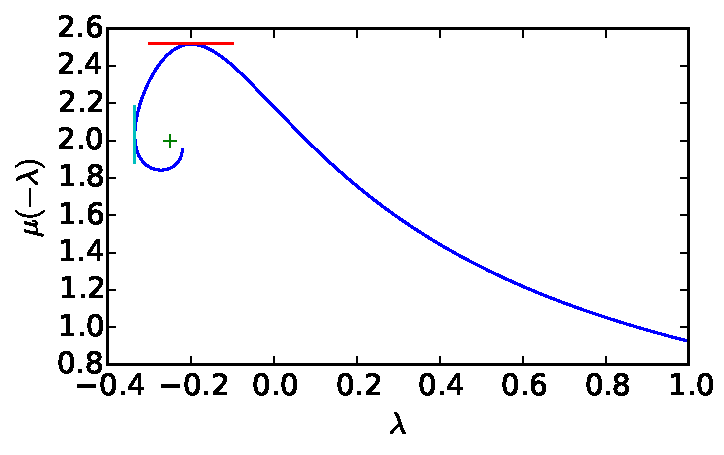
\includegraphics{calorique.pdf}
		\caption{Courbe calorique de la sphère isotherme en boîte : $\mu(\lambda)$. La croix verte représente la \textsc{sis}}
		\label{Ener}
	\end{figure}

	Dans le diagramme de Milne, la sphère isotherme singulière correspondait au point $\left(1,2\right)$.
	Dans cette nouvelle représentation elle est associée au point $\left(\lambda = \frac{3/2 - u_m}{v_m} = 1/4, \mu = v_m = 2\right)$.
	De la même manière que sur le diagramme précédent, la courbe tend en spiralant vers la sphère isotherme singulière, mais avant de l'atteindre,
	elle passe par un minimum de température, puis un maximum d'énergie délimitant ainsi des intervalles possibles d'existence d'une sphère gravitationelle isotherme en boîte.

\subsection{Stabilité de la sphère isotherme en boîte}
\subsubsection{Description statistique}
	En physique statistique, il existe deux ensembles capables de décrire la sphère isotherme telle que nous l'avons construite :
	\begin{enumerate}

		\item l'ensemble micro-canonique: nous imposons la valeur de l'énergie totale de la sphère, et
			l'équilibre est atteint pour une certaine valeur de la température. C'est par exemple le cas
			d'une sphère isotherme constituée de particules enfermées dans une boîte aux parois
			réfléchissantes. La dispersion de vitesse de ces particules, ou température cinétique du
			système, s'ajuste pour atteindre l'équilibre du viriel sans dissipation d'énergie.
		
		\item l'ensemble canonique: nous imposons la valeur de la température de la sphère, le système rejoint
			l'équilibre en ajustant son énergie totale. Ce processus peut par exemple se produire en mettant
			la sphère en contact avec un bain thermique qui imposera la température et rendra possible
			l'échange d'énergie susceptible d'atteindre l'état d'équilibre.
		
	\end{enumerate}

	Lorsque l'on progresse le long de la courbe calorique vers la partie en spirale, en partant des petites valeurs
	de $X$ i.e. les grandes valeurs de $-\lambda$, nous passons successivement par les deux points remarquables: le
	premier est caractérisé par une tangente horizontale et correspond à la valeur minimale qu'il est possible d'imposer à
	la température, le second est caractérisé par une tangente verticale et correspond à la valeur minimale de
	l'énergie susceptible d'être atteinte par une sphère isotherme de masse donnée et contenue dans une boîte de
	rayon fixé.
	
	Les deux points correspondants et leurs tangentes ont été représentés sur la courbe calorique figure~\ref{Ener}.
	
	De nombreuses analyses dynamiques ont été menées concernant ces limites
	et ont révélées un lien étroit avec la stabilité du système. Une
	approche simple de cette problématique est d'étudier le constraste de
	densité de la sphère et son influence.
	
\subsection{De l'importance du contraste de densité\label{contraste-dens-SIB}}
	La densité de la sphère isotherme s'écrit :
	\begin{align*}
		\rho(r) = \frac{m}{\alpha^3}e^{-\beta m\psi(r)}
	\end{align*}
	En dehors du cas de la \textsc{sis} cette densité est toujours finie au centre du système, nous pouvons donc former la quantité sans dimension $\rho^s(r) = \frac{\rho(r)}{\rho_0}$. Un rapide calcul montre alors que 
		\begin{align}
		\rho^s(x) = e^{-h(x)}=\frac{u(x) v(x)}{x^2}
	\end{align}
	Par définition, ou en utilisant les expressions asymptotiques de $u$ et $v$ en $x=0$, nous avons $\rho^s(0)=1$.
	Au bord du système, nous avons par contre $\rho^s(X) =u_m v_m x^{-2}$, la relation~(\ref{uv_max}) permet donc d'écrire
	\begin{align*}
		\rho^s(X) = \mu X^{-2}\left(\frac{3}{2} - \lambda\mu\right) \notag
	\end{align*}
	Nous pouvons donc former le contraste de densité entre le centre et le bord du système, il s'écrit :
	\begin{align}
		\R = \frac{\rho(0)}{\rho(R)} = \frac{\rho^s(0)}{\rho^s(X)} = \frac{X^2}{\mu\left(\frac{3}{2} - \lambda\mu\right)}
	\end{align}

	Il est possible de déterminer numériquement les coordonnées des points de tangentes remarquables et donc en déduire les valeurs correspondantes du contraste de densité :
	\begin{itemize}
		\item La tangente horizontale est obtenue pour une sphère telle que $X = 9,00$ avec $\(\lambda, \mu\) = \left(-0,199; 2,518\right)$. Son contraste de densité est de $\R^\beta_c \thickapprox 32,1$.
		\item La tangente verticale est obtenue pour une sphère telle que $X = 34,3$ avec $\(\lambda, \mu\) = \left(-0,335; 2,032\right)$. Son  contraste de densité est de $\R^H_c \thickapprox 709$.
	\end{itemize}
	
	Il est même possible d'obtenir numériquement les courbes $\lambda(\R)$ et $\mu(\R)$, c'est l'objet de la figure \ref{Cal_stab}. L'analyse de stabilité est alors possible. 
	\begin{figure}[h!]
		\centering 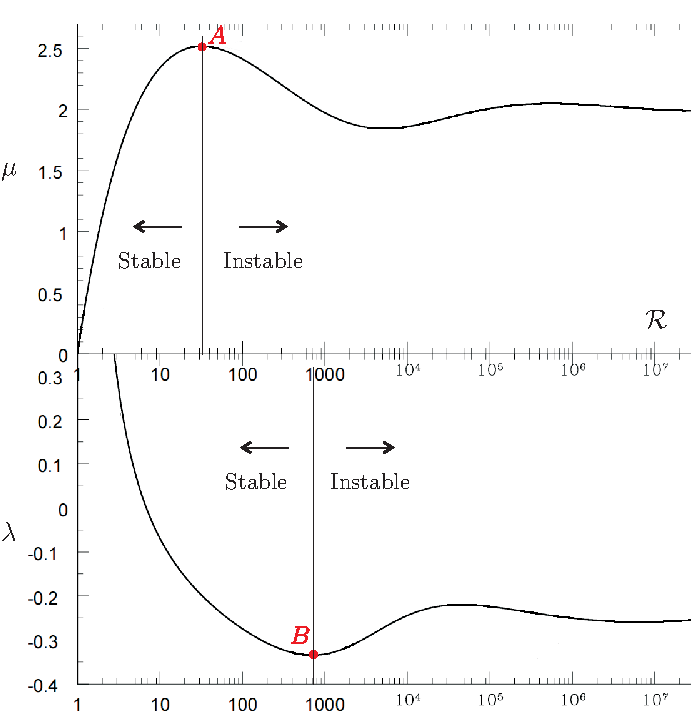
\includegraphics[scale=1.00]{graphe/calorique_stabilite.pdf}
		\caption{Courbes $\lambda(\R)$ et $\mu(\R)$ tirées de l'article \cite{2011MNRAS.414.2728Y}}
		\label{Cal_stab}
	\end{figure}
	Le maximum de l'entropie dans l'ensemble microcanonique ($\delta S=0$ avec $H=\mathrm{cte}$) dans un domaine
	borné correspond à la sphère isotherme en boite. Tous les points de la courbe $\lambda(\R)$ correspondent à
	$\delta S=0$, au point critique $B$ de coordonnées $\R=709$ et $\lambda=-0.335$ nous avons $\frac{d\lambda}{d\R}=0$ et
	$\delta^2 S=0$ (voir \cite{1968MNRAS.138..495L}, \cite{1989ApJS...71..651P} et \cite{1990PhR...188..285P}). Dans
	ces deux derniers articles Padmanabhan (\cite{1989ApJS...71..651P} et \cite{1990PhR...188..285P}) montre que
	tous les points de la courbe $\lambda(\R)$ situés avant $B$ , i.e. $\R < 709$, correspondent à des situations
	telles que $\delta^2 S>0$, ils correspondent à des maxima locaux d'entropie et sont donc des configurations
	stables. Par contre tout ceux situés après le point $B$, i.e. $\R > 709$, sont toujours instables : soit parce
	que $\delta^2 S<0$ dans un premier temps (\cite{1989ApJS...71..651P}), soit pour des raisons dynamiques plus
	compliquées (voir \cite{Katz-Stab} et \cite{1979MNRAS.189..817K}). 
	
	Comme le montre \cite{2002A&A...381..340C}, dans l'ensemble canonique la situation est différente. En lieu et
	place de l'entropie, le potentiel d'étude de la stabilité est l'énergie libre $F=H-TS$. La courbe à étudier est
	maintenant $\mu(\R)$. Elle fait apparaitre deux régions. Tous les points de cette courbe situés avant le point
	$A$ de coordonnées $\R=32,1$ et $\lambda=2,518$, i.e. $\R<32,1$, sont tels que $\delta^2 F>0$ : ils
	correspondent à des sphères isothermes en boite stables. Au delà du point $A$, i.e. $\R>32,1$, le système est
	instable dans l'ensemble canonique.
	
	De manière concrète nous retiendrons que l'étude de la stabilité d'une sphère isotherme en boite est de manière générale contrôlée par son contraste de densité et l'étude des tangentes horizontales ou verticales de sa courbe calorique.   
	\begin{itemize}

		\item Pour une boite isolée aux parois réfléchissantes (situation microcanonique), le point critique de
			stabilité est associé à la tangente verticale la plus à gauche sur la courbe calorique
			$\mu(-\lambda)$ de la figure \ref{Ener}.

		\item Pour une boite dont les parois (conductrices de chaleur...) sont en contact avec un thermostat, le
			point critique de stabilité est associé à la tangente horizontale la plus en haut sur la courbe
			calorique $\mu(-\lambda)$ de la figure \ref{Ener}.

	\end{itemize}
	
